%% chapter5_slides.tex  -  Chapter 5: Analyzing South African Equity Option
%% Prices Using Normalizing Flows
%% Bayesian Machine Learning in Quantitative Finance: Theory and Practical
%% Applications - Mongwe, Mbuvha & Marwala (Springer, 2025)
%% Compile: pdflatex -interaction=nonstopmode chapter5_slides.tex  (twice)
\documentclass[aspectratio=169,10pt]{beamer}

\usetheme{Madrid}
\usecolortheme{seahorse}
\usefonttheme{professionalfonts}

%% packages
\usepackage{amsmath,amssymb,mathtools}
\usepackage{bm}
\usepackage{graphicx}
\usepackage{booktabs}
\usepackage{array}
\usepackage{listings}
\usepackage{xcolor}
\usepackage{caption}

\graphicspath{{figures/}}

%% listings style
\lstdefinestyle{pycode}{
  language=Python,
  basicstyle=\ttfamily\scriptsize,
  keywordstyle=\color{blue!40!black}\bfseries,
  commentstyle=\color{green!50!black}\itshape,
  stringstyle=\color{orange!80!black},
  numbers=left,
  numberstyle=\tiny\color{gray},
  numbersep=5pt,
  frame=single,
  backgroundcolor=\color{gray!7},
  tabsize=2,
  showstringspaces=false,
  breaklines=true,
  captionpos=b,
}
\lstset{style=pycode}

%% footline, no navigation symbols
\setbeamertemplate{footline}[frame number]
\setbeamertemplate{navigation symbols}{}

%% macros
\newcommand{\Prob}{\mathbb{P}}
\newcommand{\Exp}{\mathbb{E}}
\newcommand{\R}{\mathbb{R}}

%%=============================================================================
\title[Bayesian ML in QF -- Ch.5]{Bayesian Machine Learning in Quantitative Finance}
\subtitle{Chapter 5: Option Prices via Normalizing Flows}
\author{Based on Mongwe, Mbuvha \& Marwala}
\date{}

%%=============================================================================
\begin{document}

\begin{frame}
  \titlepage
\end{frame}

\begin{frame}{Chapter Outline}
  \tableofcontents
\end{frame}

%%=============================================================================
\section{5.1 Introduction}
%%=============================================================================
\begin{frame}[allowframebreaks]{5.1 Introduction: Why This Chapter?}

\begin{block}{The Problem With Black--Scholes}
Geometric Brownian motion (the engine behind Black--Scholes) assumes log-returns
are Gaussian. Real equity returns are not: they show \textbf{fat tails} and a
\textbf{volatility skew} across strikes. Two classical fixes exist:
\begin{itemize}
  \item let volatility itself be stochastic (Heston model -- Chapter 4),
  \item add jumps to the price process (Merton, Kou jump-diffusion models).
\end{itemize}
Both are \emph{economically motivated}: you write down assumptions about the
world, then derive option prices from them. They are interpretable, but hard
to extend -- adding parameters can break their economic derivation.
\end{block}

\begin{block}{The Machine-Learning Alternative}
Instead of assuming dynamics, treat option pricing as a \textbf{regression
problem}: fit a flexible function $f_w(K)$ (a neural network, say) directly to
observed market prices at strikes $K$. This can fit market prices almost
perfectly, but the fitted curve is \emph{not guaranteed to be arbitrage-free} --
it might imply negative probabilities or a negative fair option price
somewhere. Custom loss penalties can discourage this, but cannot
\emph{guarantee} it.
\end{block}

\framebreak

\begin{block}{This Chapter's Idea}
Instead of modelling the price curve $f_w(K)$ directly, model the
\textbf{risk-neutral density} implied by the prices, and only afterwards
\emph{derive} the prices from that density. If the object we learn is
guaranteed to be a valid probability density, the option prices we recover
from it are \emph{automatically} arbitrage-free -- no custom penalty terms
needed. The tool used to learn this density is a \textbf{normalizing flow}.
\end{block}

\begin{block}{What This Chapter Does}
\begin{itemize}
  \item Uses the mixture-of-normalizing-flows framework of Yang \& Hospedales
  (2023), originally applied to a developed market (Apple-style US options),
  \item applies it instead to European options on the \textbf{JSE All Share
  Index} (South Africa, a developing market),
  \item compares mixtures with $1$, $8$, $15$, and $30$ normalizing-flow
  components, across five option maturities (14, 20, 30, 60, 90 days).
\end{itemize}
\end{block}

\begin{block}{Roadmap for This Chapter}
\begin{enumerate}
  \item Sec.~5.2: how a risk-neutral density is implied by option prices,
  and the no-arbitrage constraints it must satisfy.
  \item Sec.~5.3: what a normalizing flow is, and how it can represent this
  density.
  \item Sec.~5.4: the JSE data and experimental setup.
  \item Sec.~5.5--5.6: results and conclusions.
\end{enumerate}
\end{block}

\end{frame}

%%=============================================================================
\section{5.2 Risk-Neutral Density from Option Prices}
%%=============================================================================
\begin{frame}[allowframebreaks]{5.2 What Is a ``Risk-Neutral Density''?}

\begin{block}{Plain-Language Definition (read this first)}
The risk-neutral density is the probability distribution over the
\textbf{future asset price} that is \emph{implied by observed option prices}
-- it is \textbf{not} the real-world (physical) distribution of the stock
price. It is the distribution consistent with \textbf{no-arbitrage pricing}:
if you assume the market is arbitrage-free, there must exist some
probability measure under which every option's price equals the discounted
expected payoff. The remarkable fact (Breeden--Litzenberger, 1978) is that
you can \textbf{back this density out purely from how call option prices
change with strike} -- no model of the stock's dynamics is required.
\end{block}

\begin{block}{Intuition}
A call option with strike $K$ pays $\max(S_T-K,0)$ at maturity $\tau$.
Its price is
\[
C(K) = e^{-r\tau}\,\Exp^{\Prob^*}\!\big[\max(S_T-K,0)\big]
     = e^{-r\tau}\int_K^\infty (S-K)\,q(S)\,dS ,
\]
where $q(S)$ is the risk-neutral density of $S_T$. Differentiating this
integral twice with respect to $K$ removes the payoff structure and leaves
$q(K)$ itself (the classical Breeden--Litzenberger relation):
\[
q(K) = e^{r\tau}\,\frac{\partial^2 C(K)}{\partial K^2}.
\]
This is exactly \emph{why} a valid, arbitrage-free call-price curve must be
\textbf{convex} and \textbf{decreasing} in $K$ -- a probability density
cannot be negative.
\end{block}

\framebreak

\begin{block}{Carr, Geman, Madan \& Yor (2003): Static Arbitrage Conditions}
Let $f_w(K)$ be the model's fitted option-pricing function at strike $K$
(for a fixed expiry $\tau$), $F_\tau$ the forward price, $F_\tau =
\exp(-r\tau)S_0$, $r$ the continuously compounded zero-coupon rate, $S_0$
the initial stock price, and $q$ the continuous dividend yield. Any
arbitrage-free pricing curve must satisfy:
\[
\frac{\partial f_w(K)}{\partial K} \le 0 \tag{5.1}
\]
\[
\frac{\partial^2 f_w(K)}{\partial^2 K} \ge 0 \tag{5.2}
\]
\[
f_w(\infty) = 0 \tag{5.3}
\]
\[
\max\big(0,\exp(-r\tau)(F_\tau-K)\big) \le f_w(K) \ge \exp(-r\tau)F_\tau \tag{5.4}
\]
Eq.~(5.1): prices fall as strike rises. Eq.~(5.2): the curve is convex --
this is precisely the Breeden--Litzenberger non-negativity of the density
above. Eq.~(5.3): price $\to 0$ for very large strikes. Eq.~(5.4): the price
is bounded between intrinsic value and the discounted forward (as given
verbatim in the book).
\end{block}

\framebreak

\begin{block}{The Chapter's Reframing: Model the Density, Not the Price}
Yang \& Hospedales (2023) show that it is much simpler to design a
\textbf{density} that automatically satisfies all of the above than to force
a generic function $f_w$ to satisfy them. Their trick: work with the density
of \textbf{forward log-moneyness} $x = \log(S_T/F_\tau)$, called $q_w(x)$,
and \emph{define} the pricing function as
\[
f_w(K) = \exp(-r\tau)\,F_\tau \int_{-\infty}^{\infty}
   \max\!\Big(\exp(x) - \frac{K}{F_\tau},\,0\Big)\,q_w(x)\,dx. \tag{5.5}
\]
This is just the discounted expected payoff, written in log-moneyness
coordinates instead of directly in $S_T$. All four constraints (5.1)--(5.4)
now reduce to three simple conditions on the density $q_w$ itself:
\[
q_w(x) \ge 0 \tag{5.6}
\]
\[
\int_{-\infty}^{\infty} q_w(x)\,dx = 1 \tag{5.7}
\]
\[
\int_{-\infty}^{\infty} \exp(x)\,q_w(x)\,dx = 1 \tag{5.8}
\]
\end{block}

\framebreak

\begin{block}{Reading the Three Constraints}
\begin{itemize}
  \item (5.6)--(5.7): $q_w$ is a genuine probability density -- non-negative
  and integrates to one. \emph{Any} normalized density automatically
  satisfies these.
  \item (5.8): sets $\Exp[\exp(x)] = 1$. Since $x=\log(S_T/F_\tau)$, this
  means $\Exp[S_T] = F_\tau = S_0\exp((r-q)\tau)$ -- the expected asset
  price at maturity, discounted, equals today's dividend-adjusted spot. This
  is precisely the defining property of a \textbf{risk-neutral} density: the
  discounted asset price is a martingale.
\end{itemize}
So: if $q_w$ is \emph{any} density satisfying (5.8), plugging it into
(5.5) gives option prices that are \textbf{automatically arbitrage-free} --
no extra penalty terms are needed in training. This is the entire appeal of
the approach.
\end{block}

\begin{alertblock}{Concrete By-Hand Example: Finite-Difference Recovery}
Suppose (toy numbers) a call trades at $C(95)=10.13$, $C(100)=7.60$,
$C(105)=5.60$, with $\tau=0.25$, $r=5\%$, strike spacing $h=5$. The
central finite-difference estimate of the Breeden--Litzenberger second
derivative is
\[
q(100) \approx e^{r\tau}\,\frac{C(105) - 2\,C(100) + C(95)}{h^2}
       = e^{0.0125}\cdot\frac{5.60 - 2(7.60) + 10.13}{25} \approx 0.0216.
\]
This tiny hand calculation is exactly what Sec.~5.2 formalizes: \emph{the
curvature of the price curve in $K$, sampled at nearby strikes, directly
gives you the density.} The toy figure below extends this to a full strike
grid.
\end{alertblock}

\framebreak

\begin{block}{Toy Running Example: Recovering a Density from Prices}
\centering
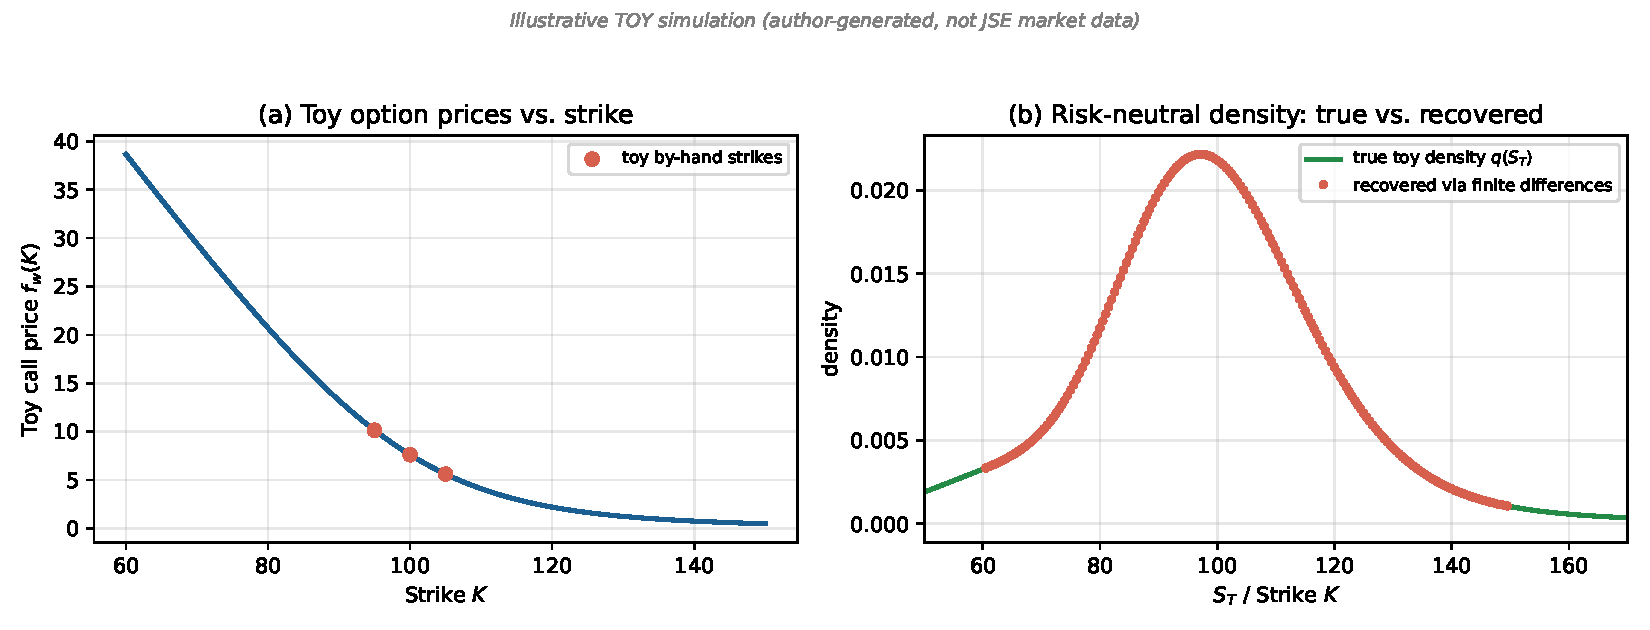
\includegraphics[width=0.92\textwidth]{option_price_and_rnd.pdf}
\end{block}
{\scriptsize A ``true'' toy risk-neutral density (mixture of two lognormals,
author-generated) is used to price toy call options across a strike grid;
finite-differencing those prices recovers the density almost exactly. This
is an illustrative simulation, not JSE market data.}

\end{frame}

%%=============================================================================
\begin{frame}[fragile]{Python: Toy Option-Price-to-Density Recovery (5.2)}
\begin{lstlisting}[style=pycode]
import numpy as np

r, tau = 0.05, 0.25          # toy rate, time to expiry
S_grid = np.linspace(1.0, 260.0, 20000)   # integration grid for S_T

def call_price(K, q_density):
    """Discounted expected payoff under a toy risk-neutral density."""
    payoff = np.maximum(S_grid - K, 0.0)
    return np.exp(-r * tau) * np.trapezoid(payoff * q_density, S_grid)

# Breeden-Litzenberger: q(K) = exp(r*tau) * d^2 C / d K^2
def implied_density(K_grid, prices, r, tau):
    h = K_grid[1] - K_grid[0]
    q = np.full_like(prices, np.nan)
    q[1:-1] = np.exp(r * tau) * (
        prices[2:] - 2 * prices[1:-1] + prices[:-2]
    ) / h**2
    return q

K_grid = np.linspace(60.0, 150.0, 181)
C_vals = np.array([call_price(K, q_true_vals) for K in K_grid])
q_recovered = implied_density(K_grid, C_vals, r, tau)
\end{lstlisting}
\end{frame}

%%=============================================================================
\section{5.3 Normalizing Flows}
%%=============================================================================
\begin{frame}[allowframebreaks]{5.3 Normalizing Flows: A Recap}

\begin{block}{Intuition (recap from Chapter 2)}
A normalizing flow builds a complicated target density out of a
\textbf{simple} base density (usually a standard Gaussian) by pushing
samples through a chain of \textbf{invertible, differentiable}
transformations. Because each step is invertible, we can track exactly how
probability mass gets stretched or compressed, and hence compute the exact
density of the transformed variable -- unlike, say, a GAN, which gives you
samples but no tractable density.
\end{block}

\begin{block}{Setup and Notation (as in the book)}
Let $x \sim q(x)$ be a sample from a simple \textbf{base distribution}
(e.g.\ standard Gaussian). Let $T$ be an invertible, differentiable
transformation. Define
\[
w = T(x).
\]
Here $w$ denotes a sample from the \textbf{target (unknown) distribution}
$p(w)$ that we want to represent -- in this chapter's application, $w$ will
play the role of the risk-neutral log-moneyness variable. The
\textbf{change-of-variables formula} gives the density of $w$ as
\[
p(w) = q(x)\,\big|\det\big(J_T(x)\big)\big|^{-1}, \tag{5.9}
\]
where $J_T(x)$ is the Jacobian matrix of $T$ evaluated at $x$. In one
dimension this is simply $p(w) = q(x)\,|T'(x)|^{-1}$.
\end{block}

\framebreak

\begin{block}{Step-by-Step Derivation of Change of Variables (1D, from scratch)}
Take a simple invertible map $f$ with $w = f(x)$, so $x = f^{-1}(w)$. We
want $p(w)$ given that $x\sim q(x)$.
\begin{enumerate}
  \item Probability is conserved under the map: for any small interval,
  $\Prob(w \in [f(x), f(x+dx)]) = \Prob(x\in[x,x+dx])$.
  \item In terms of densities: $p(w)\,|dw| = q(x)\,|dx|$.
  \item Rearranging: $p(w) = q(x)\,\left|\dfrac{dx}{dw}\right| = q(f^{-1}(w))\,\left|\dfrac{d f^{-1}(w)}{dw}\right|$.
  \item Equivalently, since $\frac{dx}{dw} = 1/\frac{dw}{dx}$: $\;p(w) = q(x)\,|f'(x)|^{-1}$.
\end{enumerate}
\textbf{Worked example:} let $f(x) = \exp(x)$, so $w = e^x$, $x=\log w$,
$f'(x) = e^x = w$. If $x\sim N(0,1)$, then
\[
p(w) = \underbrace{\frac{1}{\sqrt{2\pi}}e^{-\frac{1}{2}(\log w)^2}}_{q(x=\log w)}
        \cdot \frac{1}{w}, \qquad w>0,
\]
which is exactly the \textbf{log-normal} density -- a normalizing flow with
a single exponential layer turns a Gaussian into a log-normal.
\end{block}

\framebreak

\begin{block}{Why Flows Are Useful Here}
\begin{itemize}
  \item The base is easy to sample from and its density is known in closed
  form (Gaussian).
  \item Each layer $T$ is chosen so that $\det(J_T)$ is \emph{cheap to
  compute} -- this is the key design constraint in flow architectures.
  \item Composing many simple invertible layers, $T = T_L \circ \cdots \circ
  T_1$, lets a simple base density become arbitrarily complex, while the
  Jacobian of the composition is just the \textbf{product} of the individual
  layer Jacobians (chain rule).
\end{itemize}
\end{block}

\begin{block}{This Chapter's Flow Setup}
The chapter builds the risk-neutral density $q_w(x)$ as the pushforward of a
\textbf{one-dimensional standard Gaussian} through a normalizing flow. Write
$\gamma \sim N(0,1)$; after a sequence of invertible transforms $q_w$,
\[
\gamma \xrightarrow{\;q_w\;} x,
\]
so $x$ is a sample from the risk-neutral (log-moneyness) density. The
parameters $w$ of the flow are then fitted (Sec.~5.4) so that the option
prices implied via Eq.~(5.5) match the market, using Monte Carlo estimation
of the pricing integral. The exact flow architecture (layer types, four
layers per flow) is taken from Yang \& Hospedales (2023).
\end{block}

\framebreak

\begin{block}{Mixture of Normalizing Flows}
A single normalizing flow can struggle to represent very flexible,
multi-modal, or heavy-tailed shapes without becoming very deep. Yang \&
Hospedales (2023) instead use a \textbf{mixture} of $M$ independent
normalizing flows:
\[
q(x) = \sum_{i=1}^{M} \pi_i\, q_i(x), \qquad \pi_i > 0,\quad \sum_{i=1}^M \pi_i = 1. \tag{5.10}
\]
Each component $q_i$ is realized by its own flow, $\gamma \xrightarrow{q_{w_i}} x$.
As long as $\pi = (\pi_1,\dots,\pi_M)$ lies on the probability simplex, all
of the no-arbitrage conditions (5.6)--(5.8) continue to hold for the
mixture. The mixture creates $M$ pricing models whose outputs are
re-weighted and summed; all parameters $\{\pi, w_1,\dots,w_M\}$ are learned
jointly by gradient-based optimization.
\end{block}

\begin{block}{Toy Running Example: A 1D Flow From Scratch}
\centering
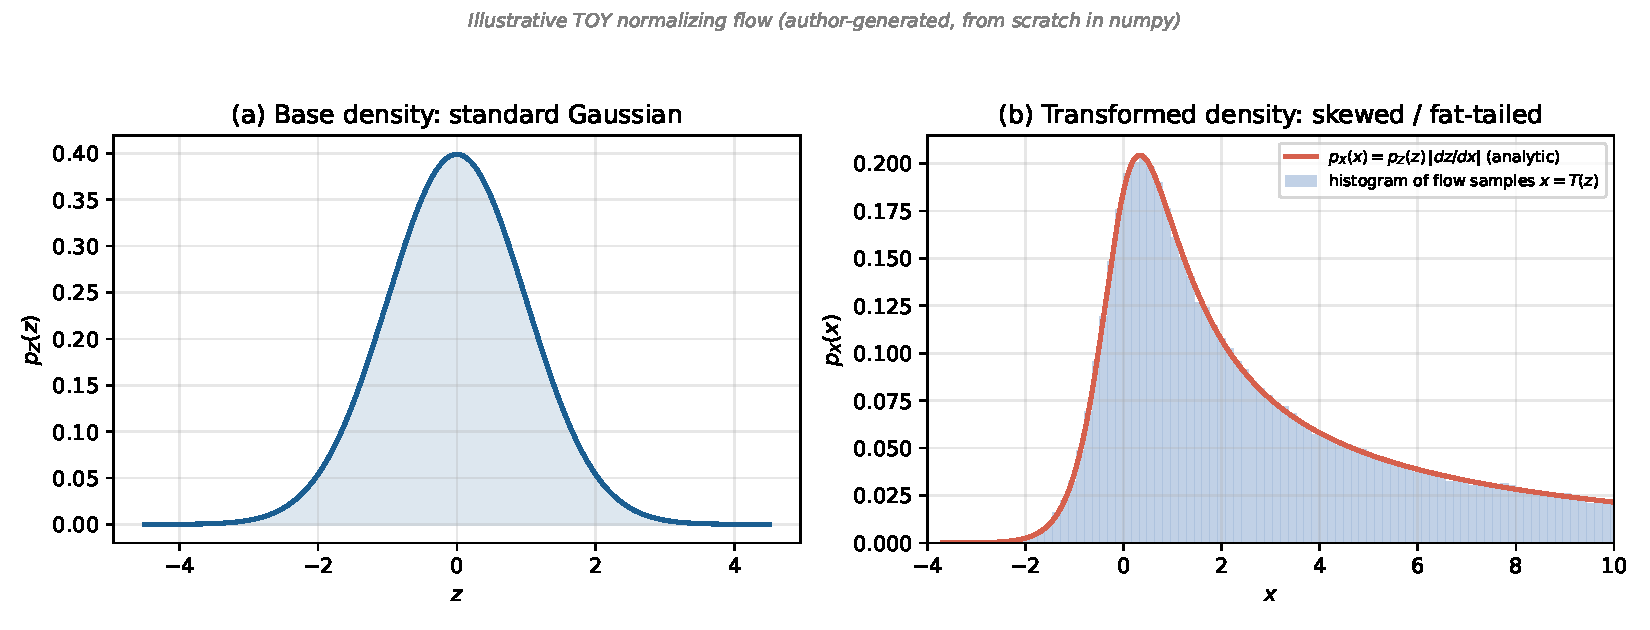
\includegraphics[width=0.85\textwidth]{normalizing_flow_toy.pdf}
\end{block}
{\scriptsize A toy two-layer flow (affine, then a monotone sinh-arcsinh
layer) transforms a standard Gaussian base into a skewed, fat-tailed target
density -- exactly the kind of shape a risk-neutral density can have.
Illustrative simulation only.}

\end{frame}

%%=============================================================================
\begin{frame}[fragile]{Python: A Toy 1D Normalizing Flow From Scratch (5.3)}
\begin{lstlisting}[style=pycode]
import numpy as np

# Two invertible layers composed: affine, then sinh-arcsinh
a, b = 1.0, 0.0          # affine layer
eps, delta = 1.0, 0.6    # sinh-arcsinh layer (skew, tail weight)

def flow_forward(z):
    u = a * z + b
    x = np.sinh((np.arcsinh(u) + eps) / delta)
    return x

def flow_forward_with_jacobian(z):
    u, du_dz = a * z + b, a                       # layer 1 + its derivative
    x = np.sinh((np.arcsinh(u) + eps) / delta)     # layer 2
    dx_du = np.cosh((np.arcsinh(u) + eps) / delta) / (delta * np.sqrt(1 + u**2))
    return x, dx_du * du_dz                        # chain rule -> dx/dz

def standard_normal_pdf(z):
    return np.exp(-0.5 * z**2) / np.sqrt(2 * np.pi)

# Change-of-variables formula: p_X(x) = p_Z(z) * |dz/dx| = p_Z(z) / |dx/dz|
z_grid = np.linspace(-4.5, 4.5, 4000)
x_of_z, dxdz = flow_forward_with_jacobian(z_grid)
p_x = standard_normal_pdf(z_grid) / np.abs(dxdz)
\end{lstlisting}
\end{frame}

%%=============================================================================
\section{5.4 Numerical Experiments}
%%=============================================================================
\begin{frame}[allowframebreaks]{5.4.1 Data Description}

\begin{block}{Intuition}
Having defined the model, we now need real market prices to fit it to. The
chapter deliberately targets a \textbf{developing-market} index (JSE) --
previous normalizing-flow work (Yang \& Hospedales, Loaiza-Ganem et al.) had
only been tested on developed markets (e.g.\ Apple options).
\end{block}

\begin{block}{The Dataset}
\begin{itemize}
  \item European options on the \textbf{JSE All Share Index}, expiring
  \textbf{22 July 2019}.
  \item Five maturities: \textbf{14, 20, 30, 60, and 90} days to expiry.
  \item A subset of the data used in Mongwe et al.\ (2022).
  \item Fields available: strikes, the \textbf{3-month JIBAR} rate (used as
  the risk-free proxy), and time to expiry, for both puts and calls.
  \item \textbf{200 call options} in total, split \textbf{90/10} into
  train and test sets.
\end{itemize}
\end{block}

\framebreak

\begin{block}{Why JIBAR and Why This Split Matters}
JIBAR (Johannesburg Interbank Average Rate) is the local benchmark rate
used in place of a risk-free rate such as LIBOR/SOFR in developed markets --
appropriate given the chapter's focus on a South African market. The
90/10 train/test split lets the chapter report genuinely \textbf{predictive}
performance: the flow mixture is fitted on 90\% of strikes and evaluated
on the held-out 10\%, which is what all reported metrics in Sec.~5.5
describe.
\end{block}

\end{frame}

%%=============================================================================
\begin{frame}[allowframebreaks]{5.4.2 Experiment Setup and Performance Metrics}

\begin{block}{Model Configurations Compared}
\begin{itemize}
  \item Mixture of normalizing flows with $M \in \{1, 8, 15, 30\}$
  components.
  \item Each individual normalizing flow has \textbf{four layers}.
  \item Architecture and layer specifications follow Yang \& Hospedales
  (2023) exactly; implementation is in Python, based on the module they
  provide.
  \item Training objective: minimize the \textbf{mean absolute error}
  between the market's actual option prices and the model's predicted
  prices (not a likelihood-only objective).
\end{itemize}
\end{block}

\begin{block}{Performance Metrics (evaluated on the held-out test set)}
\begin{itemize}
  \item \textbf{MSE} -- Mean Squared Error: $\frac{1}{n}\sum_i (y_i - \hat y_i)^2$,
  penalizes large errors heavily.
  \item \textbf{MAE} -- Mean Absolute Error: $\frac{1}{n}\sum_i |y_i - \hat y_i|$,
  robust to outliers, and also the training loss used here.
  \item \textbf{$R^2$} -- coefficient of determination: fraction of variance
  in market prices explained by the model (closer to 1 is better).
  \item \textbf{MAPE} -- Mean Absolute Percentage Error: error scaled by the
  price level, useful for comparing across strikes of very different
  price magnitude.
\end{itemize}
\end{block}

\framebreak

\begin{block}{What to Watch For in the Results}
Because there are five maturities $\times$ four mixture sizes $\times$ four
metrics, the natural question when reading Sec.~5.5 is: \emph{does one
mixture size dominate across all expiries, or does the best choice depend on
time to expiry?} Keep this question in mind -- it is exactly what the
chapter's headline finding addresses.
\end{block}

\end{frame}

%%=============================================================================
\section{5.5 Results and Discussions}
%%=============================================================================
\begin{frame}[allowframebreaks]{5.5 Results: Performance Tables}

\begin{block}{Reading the Tables}
Tables 5.1--5.5 report R2, MSE, MAPE, and MAE on \textbf{unseen (test)}
JSE All Share Index option data, for the 14-, 20-, 30-, 60-, and 90-day
expiries respectively, across the $1$/$8$/$15$/$30$-component mixtures.
Bold entries mark the best (outperforming) model for that metric. These are
the book's actual reported numbers.
\end{block}

\begin{table}
\centering
\scriptsize
\begin{tabular}{lrrrr}
\toprule
Metric (14-day) & 1 mixture & 8 mixture & 15 mixture & 30 mixture \\
\midrule
R2   & 0.99936833 & 0.99925830 & 0.99963457 & \textbf{0.99989999} \\
MSE  & 0.00131217 & 0.00154073 & 0.00075910 & \textbf{0.00020792} \\
MAPE & 0.14248936 & 0.17627028 & 0.14951472 & \textbf{0.07344729} \\
MAE  & 0.02642767 & 0.02970133 & 0.02282180 & \textbf{0.01126697} \\
\bottomrule
\end{tabular}
\caption*{Table 5.1: 14-day options.}
\end{table}

\begin{table}
\centering
\scriptsize
\begin{tabular}{lrrrr}
\toprule
Metric (20-day) & 1 mixture & 8 mixture & 15 mixture & 30 mixture \\
\midrule
R2   & 0.99738186 & 0.99874109 & 0.99967048 & \textbf{0.99983906} \\
MSE  & 0.00496526 & 0.00238749 & 0.00062491 & \textbf{0.00030521} \\
MAPE & 0.29285721 & 0.11292648 & 0.05536494 & \textbf{0.03841418} \\
MAE  & 0.05339091 & 0.03505068 & 0.01846331 & \textbf{0.01131606} \\
\bottomrule
\end{tabular}
\caption*{Table 5.2: 20-day options.}
\end{table}

\framebreak

\begin{table}
\centering
\scriptsize
\begin{tabular}{lrrrr}
\toprule
Metric (30-day) & 1 mixture & 8 mixture & 15 mixture & 30 mixture \\
\midrule
R2   & 0.99941305 & \textbf{0.99990101} & 0.99938930 & 0.99984136 \\
MSE  & 0.00148616 & \textbf{0.00025062} & 0.00154610 & 0.00040166 \\
MAPE & 0.08995644 & 0.02934196 & 0.03757242 & \textbf{0.02122791} \\
MAE  & 0.03490084 & \textbf{0.01289784} & 0.02974536 & 0.01489130 \\
\bottomrule
\end{tabular}
\caption*{Table 5.3: 30-day options.}
\end{table}

\begin{table}
\centering
\scriptsize
\begin{tabular}{lrrrr}
\toprule
Metric (60-day) & 1 mixture & 8 mixture & 15 mixture & 30 mixture \\
\midrule
R2   & 0.99065079 & \textbf{0.99964408} & 0.99750925 & 0.99921971 \\
MSE  & 0.01183464 & \textbf{0.00045052} & 0.00315288 & 0.00098771 \\
MAPE & 0.11747006 & \textbf{0.01410177} & 0.07385365 & 0.02503132 \\
MAE  & 0.08086322 & \textbf{0.01507402} & 0.04882987 & 0.02420844 \\
\bottomrule
\end{tabular}
\caption*{Table 5.4: 60-day options.}
\end{table}

\framebreak

\begin{table}
\centering
\scriptsize
\begin{tabular}{lrrrr}
\toprule
Metric (90-day) & 1 mixture & 8 mixture & 15 mixture & 30 mixture \\
\midrule
R2   & 0.99713960 & \textbf{0.99956541} & 0.99905050 & 0.99806153 \\
MSE  & 0.00518381 & \textbf{0.00078761} & 0.00172074 & 0.00351303 \\
MAPE & 0.10925920 & \textbf{0.01698751} & 0.03629014 & 0.03546318 \\
MAE  & 0.06111890 & \textbf{0.02207337} & 0.03577344 & 0.04499231 \\
\bottomrule
\end{tabular}
\caption*{Table 5.5: 90-day options.}
\end{table}

\framebreak

\begin{block}{Headline Finding: Best Mixture Size Depends on Expiry}
\begin{itemize}
  \item For \textbf{14-} and \textbf{20-day} options: the \textbf{30-component}
  mixture wins on every metric, with the \textbf{15-component} mixture a
  close second.
  \item For \textbf{30-}, \textbf{60-}, and \textbf{90-day} options: the
  \textbf{8-component} mixture wins on (almost) every metric instead.
  \item The \textbf{single-flow} ($M=1$) model is, on average, the
  \textbf{worst} performer -- confirming that some degree of mixing helps.
\end{itemize}
\end{block}

\begin{block}{Why Does Expiry Matter? -- The Kink Argument}
As expiry approaches, a call's payoff as a function of strike develops a
sharper \textbf{kink} (the option value hits exactly zero for large
strikes). Capturing this increasingly non-linear payoff shape requires
\textbf{more} mixture components. Conversely, options far from expiry have
an almost \textbf{straight-line} payoff-versus-strike relationship, which a
handful of components can already capture well. This is why short-dated
options favour large mixtures (30) while longer-dated options are well
served by a moderate mixture (8).
\end{block}

\framebreak

\begin{block}{Qualitative Picture From Figures 5.1--5.5}
\begin{itemize}
  \item Across all five maturities, predicted option prices from every
  mixture size visually track the market data closely as a function of
  strike (a smooth, decreasing, convex curve, as required by
  Eqs.~5.1--5.2).
  \item However, no model fits the market \textbf{perfectly}: the absolute
  error plots show non-zero errors throughout.
  \item \textbf{Errors are largest at small strikes} (where option prices
  themselves are large -- deep in-the-money) and \textbf{smallest at large
  strikes} (where option prices approach zero -- deep out-of-the-money).
  This is a consistent pattern across all maturities and mixture sizes.
\end{itemize}
\end{block}

\begin{block}{Practical Takeaway}
Because the risk-neutral density is modelled directly, and the pricing
function is derived from it via Eq.~(5.5), every model configuration
studied here is \textbf{automatically arbitrage-free} -- no custom
penalty terms were needed to enforce Eqs.~(5.1)--(5.4), unlike direct
neural-network regression of $f_w(K)$.
\end{block}

\end{frame}

%%=============================================================================
\section{5.6 Conclusions}
%%=============================================================================
\begin{frame}[allowframebreaks]{5.6 Conclusions}

\begin{block}{Summary}
\begin{itemize}
  \item This chapter analyzed JSE All Share Index option prices across five
  maturities and many strikes using a \textbf{mixture-of-normalizing-flows}
  model of the risk-neutral density.
  \item Modelling the density directly (rather than the price curve)
  \textbf{guarantees} the no-arbitrage conditions of Carr et al.\ (2003)
  are satisfied.
  \item The fitted mixtures track observed market prices well across all
  maturities and strikes.
  \item \textbf{Largest errors} occur at \textbf{small strikes}; \textbf{smallest
  errors} occur at \textbf{large strikes}.
  \item The \textbf{best number of mixture components depends on time to
  expiry}: more components help for options close to maturity (sharper
  payoff kink), fewer components suffice for options far from maturity
  (near-linear payoff).
  \item A single normalizing flow ($M=1$) consistently \textbf{underperforms}
  any mixture.
\end{itemize}
\end{block}

\begin{block}{Open Directions Noted by the Authors}
\begin{itemize}
  \item Developing a principled method to \textbf{select the optimal number
  of mixture components}, rather than trying a fixed grid $\{1,8,15,30\}$.
  \item \textbf{Jointly} modelling the risk-neutral density across \emph{all}
  maturities and strikes simultaneously (i.e., the full option price
  \textbf{surface}), instead of fitting one density per expiry.
\end{itemize}
\end{block}

\begin{alertblock}{Looking Ahead}
The next chapter (Chapter 6) shifts topic entirely: it models corporations'
\textbf{credit ratings} using \textbf{distributed Gaussian processes} --
motivated by how strongly credit ratings affect the interest rate at which
an entity can borrow.
\end{alertblock}

\end{frame}

\end{document}
